\chapter{Data Processing}

Data may be processed in either \textbf{batch} or \textbf{real-time} (\textit{stream}) fashion, or a combination of both. Batch processing is used when data can be collected and processed in a single operation, while real-time processing is used when data must be processed as soon as it is generated.

\section{Batch Processing}
This approaches relaxes the need for producing results as soon as data arrives, storing it in a buffer to later process it in chunks.

Batch processing is typically cheaper and easier to implement than real-time processing, but it may not be suitable for all use cases, but is very effective for data transformations, generate reports, and other tasks that do not require immediate results.

We have high latency, but also high throughput, and the system is easier to reason about, however, \ul{it lacks the ability for real-time decision making}.

The key paradigm here is clearly MapReduce, and the key frameworks are Hadoop and Spark.

\section{Stream Processing}

Here the focus is on processing data as soon as it is generated, providing low-latency results, and thus enabling near-real-time processing.


Data consistency refers to the accuracy and correctness of data over time.
In stream processing, \ul{data consistency is crucial to ensure that real-time analytics are accurate and reliable}. 
There are three main types of data consistency models used in stream processing systems:
\begin{itemize}
   \item \textbf{Exactly-once} processing ensures that each data item is processed exactly once, preventing duplicates or omissions. This is the most desirable level of consistency, but it can be challenging to achieve in distributed systems.
   \item \textbf{At-least-once} processing guarantees that each data item is processed at least once, but it may be processed multiple times, leading to potential duplicates.
   \item \textbf{At-most-once} processing ensures that each data item is processed at most once, but it may be lost if there are failures in the system.
\end{itemize}


\subsection{Time semantics}
\begin{itemize}
   \item \textit{Event} time - the time when the event occurred.
   \item \textit{Processing} time - the time when the event is processed. 
   \item \textit{Ingestion} time - the time when the event was received. 
\end{itemize}

Watermarks are used to track the progress of event time, and to determine when to emit results. In general aim to manage late-arrive data.

In \textbf{Stream} processing there are \ul{\textbf{Transactions}, which are atomic operations between streams}.
Clearly it may happen also that \ul{events arrive out of order}, and we need to handle this, either by buffering to wait for more data, or by allowing lateness in \textit{windowing}.

\begin{itemize}
	\item \textbf{Time-based windowing} is used to group events into windows based on time, and to process them in parallel. Windows can be fixed or sliding, and can be based on event time or processing time.
	\item \textbf{Count-based windowing} instead is used to group events into windows based on the number of events, but the same principles apply.
	\item \textbf{Session-based windowing} groups events based on inactivity periods.
\end{itemize}

\subsection{Lambda architectures}

\begin{figure}[htbp]
   \centering
   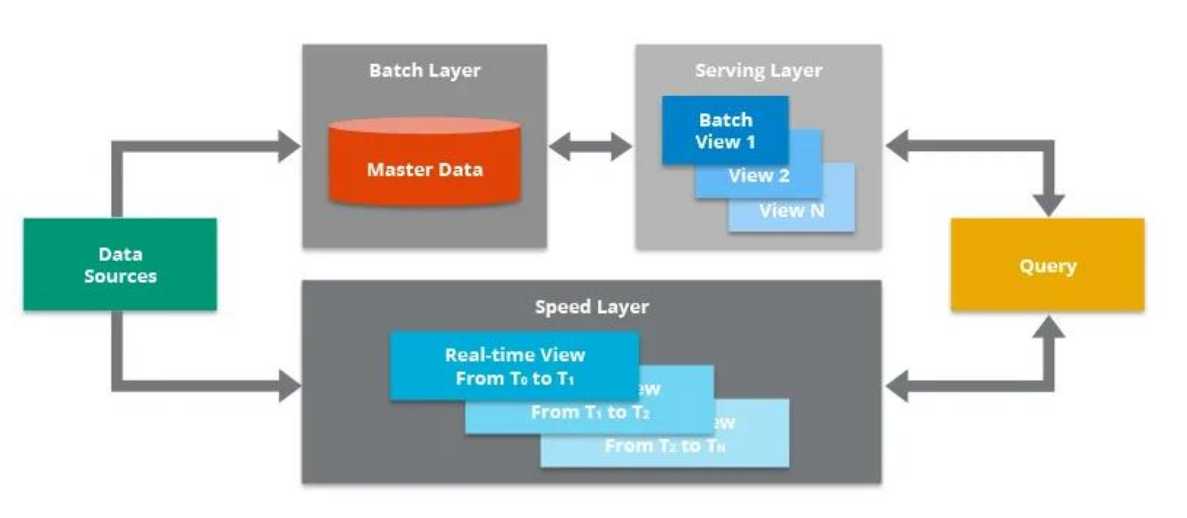
\includegraphics{images/17/lambdaarchitecture.png}
   \caption{Lambda architecture schema}
   \label{fig:17/lambdaarchitecture}
   Data sources simultaneously feed both the batch layer and the speed layer. The batch layer processes the data in large chunks, while the speed layer processes the data in real-time.
   The serving layer then combines the results from both layers to provide a unified view of the data to the end-users.
   It gets data directly from the batch layer, while it uses queries to the speed layer to get real-time updates.

\end{figure}

A \textbf{lambda architecture} is a data processing architecture designed to handle massive quantities of data by taking advantage of both \textit{batch} and \textit{stream} processing methods. 
{It consists of three layers:\ns
\begin{itemize}
   \item The \textbf{batch layer} is responsible for processing large volumes of data in a fault-tolerant and scalable manner. It is used to generate views of the data that can be queried by the serving layer.
   \item The \textbf{speed layer} is responsible for processing real-time data in a low-latency manner. It is used to generate real-time views of the data that can be queried by the serving layer.
   \item The \textbf{serving layer} is responsible for serving queries on the views generated by the batch and speed layers. It is used to provide real-time access to the data to the end-users through APIs and various tools.
\end{itemize}
}

The architecture provides a unified view
of both batch (hence, historical) and real-time data
processing, possibly handling large volumes of data and scaling horizontally.
However it may be complex to implement and maintain, and may generate redundant data processing and storage costs.


\subsection{Kappa architectures}
Lambda difficulties in implementation led to the development of \textsc{Kappa}, which simplifies the architecture by removing the batch layer, focusing on streams, ultimately offering better scaling and fault tolerance than lambda.\\
\textsc{Kappa} relies on recomputing state from streams rather than storing it.
It exploits checkpointing and state backends to manage state.

\textsc{Kappa} is very well suited for processing data from IoT devices, or analytics in general.

A \textsc{Kappa} architecture is a data processing architecture designed to handle massive quantities of data by taking advantage of stream processing methods. It consists of a single layer that processes both batch and real-time data in a fault-tolerant and scalable manner.

It is still more complex than traditional stream processing techniques, but it is more efficient and scalable.


\newpage
\subsection{CQRS - Command Query Responsibility Segregation}


\begin{paracol}{2}
   
   \begin{figure}[htbp]
      \centering
      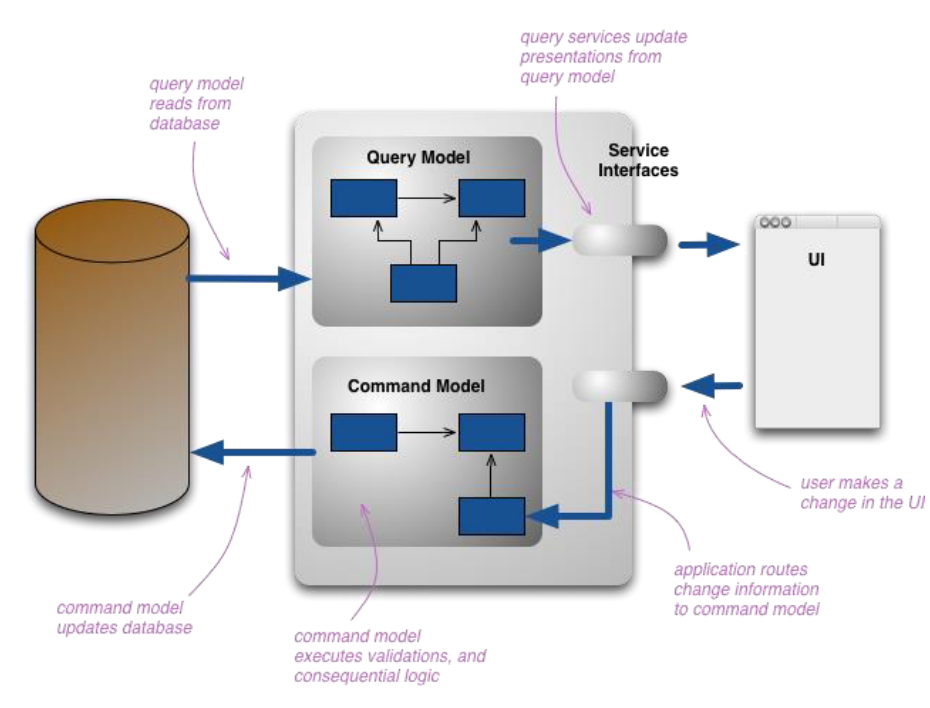
\includegraphics[width=0.95\columnwidth]{images/17/cqrs.png}
      \caption{CQRS architecture}
      \label{fig:17/cqrs}
   \end{figure}

   \switchcolumn
   \colfill

   What happens if i have many writes and few reads?
   
   {\textbf{Command Query Responsibility Segregation} (\texttt{CQRS}) is a design pattern that separates the read and write operations of a system into two separate components, along with a UI to interact with them:\ns
   \begin{itemize}
      \item The \textbf{command model} (write) is responsible for handling the write operations of the system, such as creating, updating, and deleting data.
      \item The \textbf{query model} (read) is responsible for handling the read operations of the system, such as retrieving data.
   \end{itemize}}
   This allows for better scalability, performance, and maintainability of the system.
   
   This looks good on the paper, but it is not always easy to implement, and may lead to inconsistencies between the read and write models, alongside with latency and communication overhead.
   \colfill
\end{paracol}

\section{Data Processing Frameworks}

% Wrap-up table

\begin{table}[htbp]
\centering
\scriptsize
\setlength{\arrayrulewidth}{0.8pt}
\renewcommand{\arraystretch}{1.3}
\resizebox{\textwidth}{!}{%
\begin{tabular}{|>{\raggedright\arraybackslash}p{1.8cm}|>{\raggedright\arraybackslash}p{2.8cm}|>{\raggedright\arraybackslash}p{2.8cm}|>{\raggedright\arraybackslash}p{2.8cm}|>{\raggedright\arraybackslash}p{2.8cm}|}
\hline
\textbf{Feature} & \textbf{Lambda Architecture} & \textbf{Kappa Architecture} & \textbf{CQRS} & \textbf{Shared-Nothing Architecture} \\
\hline
\textbf{Description} & Combines batch and stream processing for unified data views. & Focuses solely on stream processing, eliminating batch layers. & Separates read (queries) and write (commands) operations. & Decentralized nodes with no shared resources. \\
\hline
\textbf{Primary Use Case} & Mixed workloads requiring both batch and real-time data processing. & Real-time data streams, such as IoT or continuous analytics. & Systems with high read/write loads or complex domain logic. & Large-scale distributed systems requiring high scalability. \\
\hline
\textbf{Key Components} & Batch Layer, Speed Layer, Serving Layer. & Stream Processor, State Management, Event Logs. & Command Model, Query Model, Event Store. & Independent nodes, Partitioned Data, Local State. \\
\hline
\textbf{Data Consistency} & Consistency eventually across batch and stream layers. & Eventual consistency in state and data views. & Separate consistency models for commands and queries. & Relies on consistency protocols (e.g., eventual or strong). \\
\hline
\textbf{Scalability} & High scalability but requires coordination across layers. & Naturally scalable due to single data pipeline. & High scalability with independent query and write paths. & Horizontal scalability with no shared bottlenecks. \\
\hline
\textbf{Latency} & Low for speed layer; higher for batch processing. & Low latency, designed for real-time processing. & Low latency for reads, but can have write overhead. & Minimal latency in read/write, depends on partitioning. \\
\hline
\textbf{Fault Tolerance} & High, with redundancy in both batch and stream layers. & High, with focus on replaying events for state recovery. & Fault tolerance depends on event sourcing mechanisms. & High, as nodes operate independently. \\
\hline
\textbf{Complexity} & High, due to the need to manage two processing layers. & Moderate, simpler than Lambda but requires stream expertise. & High, due to synchronization between command and query models. & High, complexity in partitioning and load balancing. \\
\hline
\textbf{Advantages} & Unified view of historical and real-time data. & Simplified architecture with real-time focus. & Optimized read/write paths; flexibility in scaling. & High scalability and resilience; no single point of failure. \\
\hline
\textbf{Disadvantages} & Complexity in maintenance; redundant storage. & Limited to real-time use cases; relies heavily on logs. & Higher implementation cost; requires expertise. & Difficult to ensure consistency and partitioning strategy. \\
\hline
\textbf{Examples} & Log analysis, fraud detection, hybrid analytics. & IoT sensor data processing, real-time analytics. & E-commerce systems, banking transaction systems. & Global-scale distributed databases (Cassandra, DynamoDB). \\
\hline
\textbf{Best For} & Scenarios needing both batch and real-time processing. & Systems requiring low-latency, real-time stream data. & High-volume, complex, or read-heavy applications. & Large-scale distributed systems with decentralized data. \\
\hline
\end{tabular}%
}
\caption{Comparison of Data Processing Architectures}
\label{tab:dataprocessingarchitectures}
\end{table}



\subsection{Sharing or not}

In shared-nothing architectures each node is self-sufficient, has its own private memory and storage, and communicates with others using message passing.\\
These are typically used in big data processing and web applications, as they easily allow horizontal scaling.

Examples of shared-nothing architectures are Hadoop, DynamoDB, Couchbase, and Facebook TAO.

\subsection{Data Lakehouse}

This is a modern data architecture that combines the best features of data lakes and data warehouses. It allows for the storage of raw data in a data lake, and the processing of that data in a data warehouse.

A data lake is a centralized repository that allows for the storage of \textit{structured and unstructured} data at any scale. Its main use cases include data archiving, big data analytics, and machine learning.\\
A data warehouse, instead, is a centralized repository that allows for the storage of \textit{structured and processed data from multiple sources}. Its main use cases include business intelligence, reporting, and data analysis.
Differently from the data lake, the main focus of a data warehouse is on data quality, consistency, and performance, while a data lake is more about storing large volumes of raw data for future processing.


This architecture provides unified approach for structured, unstructured, and semi-structured data, and allows for the use of both batch and real-time processing methods.

An example is \textsc{Snowflake}, which is a cloud-based data warehouse that supports both batch and real-time processing methods.

\subsubsection{Data Mesh}
Data Mesh is a modern architectural approach designed to address the challenges of managing large-scale
and complex data systems, especially in distributed organizations. It emphasizes decentralization, domain-driven design, and treating data as a product.
\note{
\begin{itemize}
	\item Decentralization: Data responsibility is distributed across domain teams, avoiding a centralized data teamas a bottleneck.
	\item Interoperability: Data products across domains are designed to be interoperable.
	\item Scalability: Scales naturally with organizational and data growth.
	\item Data Discovery: Metadata and catalogs help discover data assets.
	\item Automation: Strong reliance on automation for deploying and managing data pipelines.
	\item Example - Netflix, to provide teams with the autonomy to own their datasets while maintaining consistency and governance
\end{itemize}}

\subsubsection{Choosing the right architecture}

\begin{itemize}
	\item \textbf{Lambda Architecture}: Best for systems needing both real-time and historical data processing.
	\begin{itemize}
		\item \textit{Example}: Log analysis systems combining real-time alerts and long-term trend reports.
	\end{itemize}
	
	\item \textbf{Kappa Architecture}: Ideal for real-time data applications with high throughput.
	\begin{itemize}
		\item \textit{Example}: IoT sensor data processing, where insights must be generated continuously.
	\end{itemize}
	
	\item \textbf{CQRS}: Suitable for applications with distinct read and write patterns, or complex domain logic.
	\begin{itemize}
		\item \textit{Example}: E-commerce platforms with high read traffic (product browsing) and write operations (orders).
	\end{itemize}
	
	\item \textbf{Shared-Nothing Architecture}: Perfect for distributed systems needing extreme scalability.
	\begin{itemize}
		\item \textit{Example}: Global-scale applications like social networks or e-commerce backends.
	\end{itemize}
\end{itemize}

\subsection{Federated Learning}

With federated learning, the model is trained on the edge devices, and the updates are sent to a central server. This allows for better privacy and security, as the data never leaves the edge devices.

This approach is well suited for IoT devices, as it allows for the training of models on the edge devices, and the updates are sent to a central server for aggregation.

\subsection{Serverless Data Processing}
Abstracts infrastrcture management, and allows for the deployment of data processing pipelines without the need to manage servers.
This paradigm is increasingly applied to data
processing workflows.

The key difference with traditional architectures is that serverless computing automatically manages the allocation of compute resources, scaling them up or down based on demand.
There is no need to provision or manage servers, as the cloud provider takes care of that.
 